\chapter{Graphen}
% 2te Satz verbessern
Um Pfadplanung zu entwerfen, braucht man nat"urlich auch Pfadfindung. Dazu sind Graphen wichtig, weil durch ihre Traversierung einen Pfad gefunden werden kann. Laut \cite{Turau:15} bestehen gewichtete Graphen aus Knoten, Kanten und den Kosten, die in Pfadfindungsalgorithmen genutzt werden. Kanten k"onnen nur eine Richtung haben, was sie unidirektional statt bidirektional macht. Dies ist hilfreich f"ur die Unterscheidung zwischen ausgehenden und eingehenden Kanten.

\begin{figure} %Von Website
	\centering
	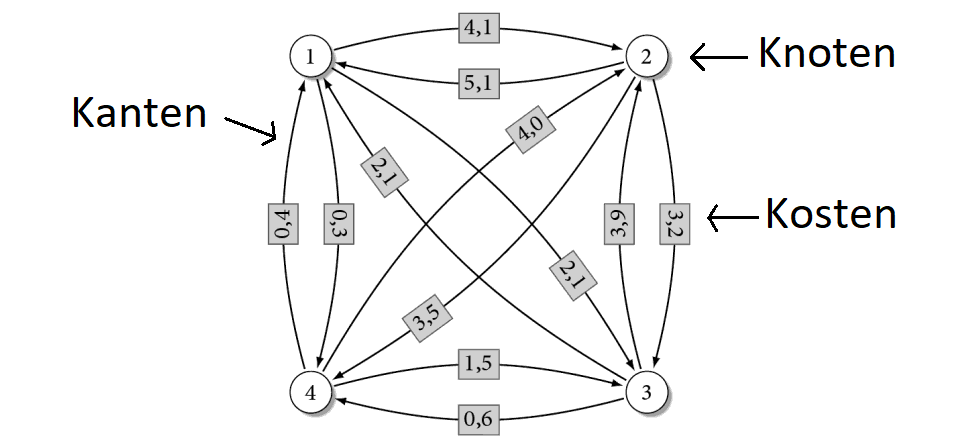
\includegraphics[width=0.9\textwidth]{images/kk_graph_S6.png}
	\caption{Abb. 1.5 von \cite[~S. 6]{Turau:15}. Gewichteter Graph mit Kantenkosten.}
	\label{sec0a}
\end{figure}

\section{B"aume}
Laut \cite{Turau:15} sind B"aume Graphen, die h"aufig f"ur Darstellung von hierarchischen Relationen genutzt werden. Ein Baum mit $m$ Knoten hat $m-1$ Kanten.\\
Gegeben ist ein Baum mit Wurzel $w$. Die Tiefe eines Knotens $e$ ist die Anzahl der Kanten von $w$ nach $e$. Die Wurzel $w$ hat Tiefe 0. Die H"ohe des Baumes ist das maximale Tiefe seiner Knoten. In Beispiel aus Abb. \ref{sec0b} ist die H"ohe des Baumes 3 und die Tiefe des Knotens $e$ ist 2.

\begin{figure} %Von Website
	\centering
	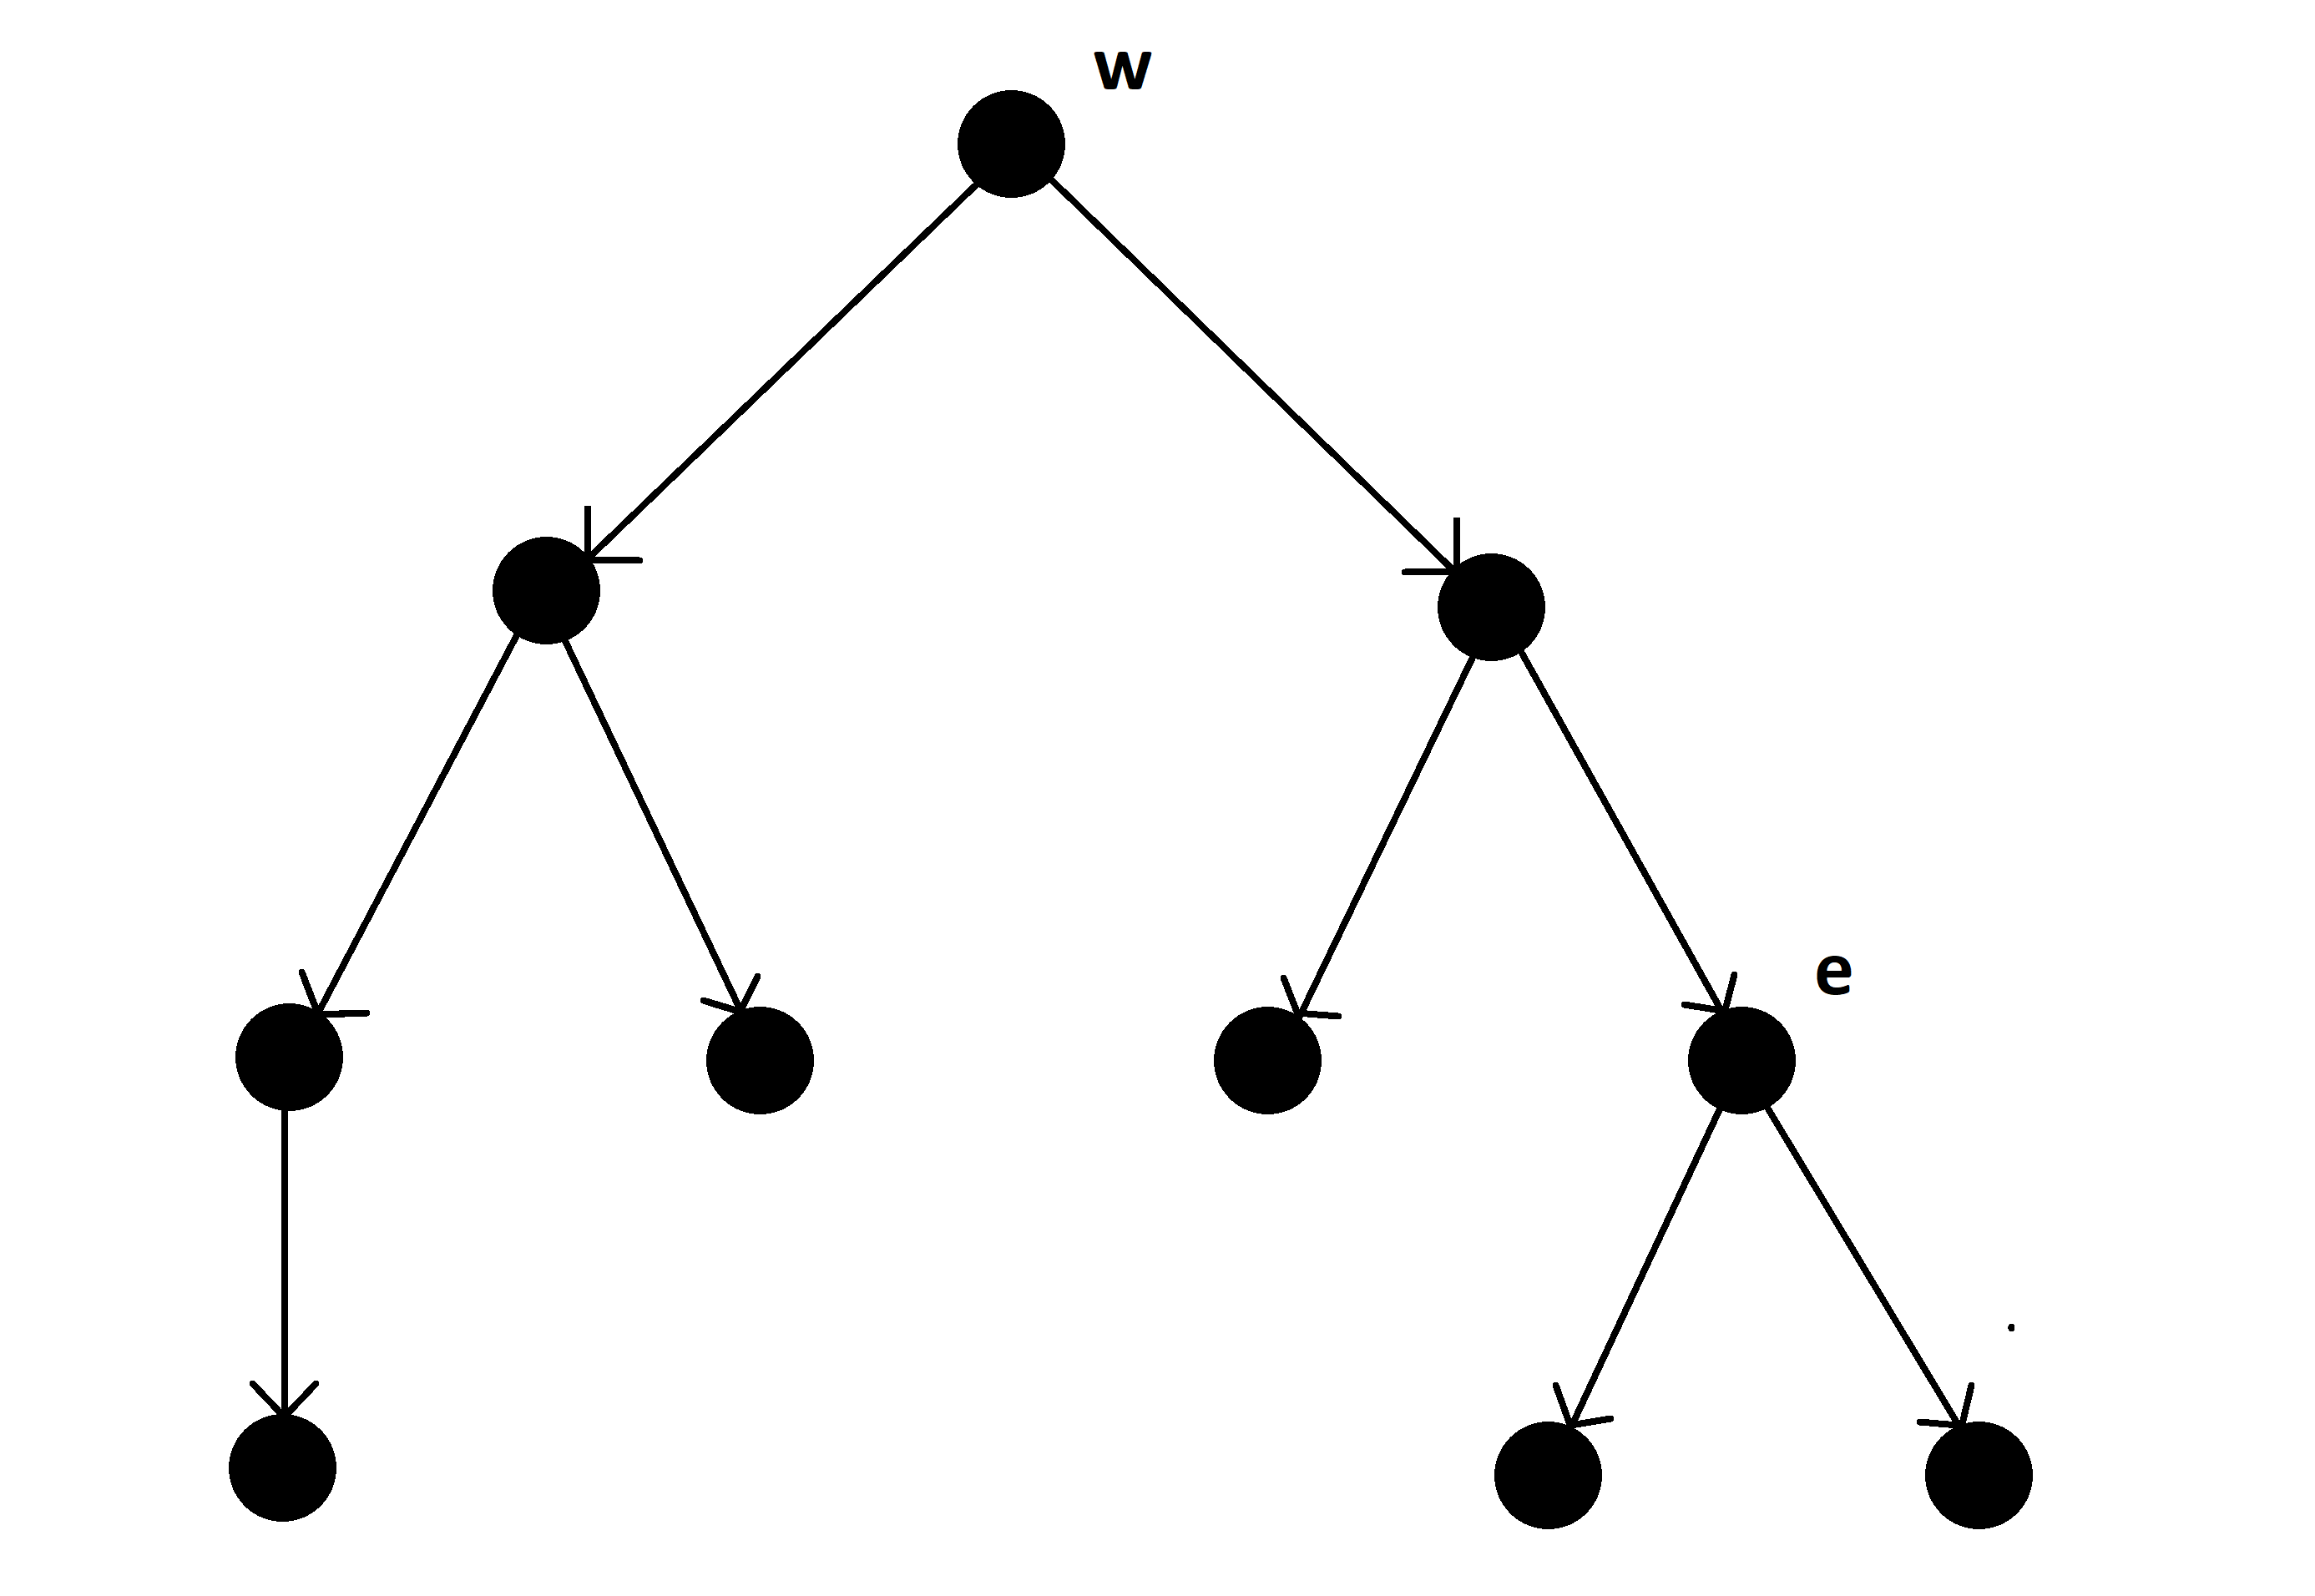
\includegraphics[width=0.6\textwidth]{images/Tree_Graph.png}
	\caption{Ein Baum mit Wurzel \textit{w}}
	\label{sec0b}
\end{figure}

\section{Navigationsnetze (\textit{eng.} Navigation Meshes)}
%\cite{Mesh:11}
%A common strategy for efficiently computing realistic
%paths is to partition the environment into a collection of
%walkable areas. This partition is often referred to as a
%navigation mesh. A useful data structure that can be used to
%construct a navigation mesh is the medial axis. The medial
%axis is the set of all points in an environment that have
%more than one distinct closest point on the boundary of the
%environment
%\cite{Mesh:16}
%(91)
%The behavior of characters may also include crawling, running, and other
%surface-based movement, but we will speak of walking and walkable
%surfaces for simplicity. The walkable surfaces of an environment
%form the free space Efree, which is usually less complex than
%the environment itself.
%A navigation mesh is a representation of Efree as a set of (usually
%polygonal) regions, along with a graph that describes how these
%regions are connected.
%(92)
%Let n be the number of vertices required to define Eobs or Efree
%using simple polygons. We call n the complexity of E.
%(93)
%A walkable environment (WE) is a set of interior-disjoint polygons
%in R3 on which characters can stand and walk. Thus, a WE is a
%clean representation of the free space Efree of a 3DE, based on the
%filtering parameters and character properties mentioned earlier. Any
%two polygons are directly connected if and only if characters can
%walk directly between them.
%
%Now that we have a definition of the free space Efree, we can define
%a navigation mesh as a tupleM= (R; G):
% R = fR0;R1; : : :g is a collection of geometric regions in R3
%that represents Efree. Each region Ri is P-simple, by which
%we mean that a region cannot intersect itself when projected
%onto the ground plane P.
% G = (V;E) is an undirected graph that describes how characters
%can navigate between the regions in R.
%Proper Work
%(91,93) \cite{Mesh:16}
%A Navigation mesh is a representation of the free space as polygonal areas alongside a navigation graph that describes how they are connected. The polygonal areas are the regions where an actor can move, refered to as walkable areas. The navigation graph describes how said actor can move to the next area, as in any surface based movement such as walking. As well as providing the requirements for path planning. pathfinding A navigation mesh can be applied to 3D and 2D environments.
%(91,93)
Nach \cite{Mesh:16} ist ein Navigationsnetz eine Darstellung des freien Raums, als polygonale Bereiche. Ein Navigationsgraph definiert die Verbindungen zwischen den Gebieten. Die polygonalen Bereiche sind die Regionen, in denen sich ein Akteur bewegen kann, und werden als begehbare Fl"achen (\textit{eng. walkable areas}) bezeichnet. Der Navigationsgraph beschreibt, wie sich der Akteur in den n"achsten Bereichen bewegen kann. Dies tritt bei jeder oberfl"achen-basierten Bewegung auf, beispielsweise Gehen oder Rennen. Ein Navigationsnetz kann sowohl auf 3D- als auch auf 2D-Umgebungen angewendet werden.

\begin{figure}[H] %Von Website
	\centering
	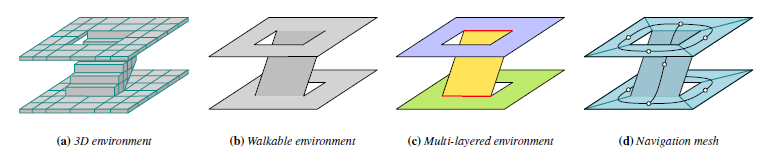
\includegraphics[width=\textwidth]{images/navigation_mesh_16.png}
	\caption{Von \cite[~S. 93]{Mesh:16} \textit{Figur 2}. Verschiedene Darstellungen einer Umgebung und ein Beispiel f"ur ihr Navigationsnetz. (a) Eine 3D-Umgebung besteht aus unbearbeitete 3D-Geometrie. (b) Der freie Raum einer 3D-Umgebung. Eine begehbare Umgebung enth"alt nur begehbare Oberfl"achen. (c) Eine mehrschichtige Umgebung ist in Schichten unterteilt. (d) Ein Navigationsnetz ist eine Beschreibung, einer begehbaren Umgebung f"ur Pfadplanungszwecke.}
	\label{sec1a}
\end{figure}
\begin{figure}[H] %Von Website
	\centering
	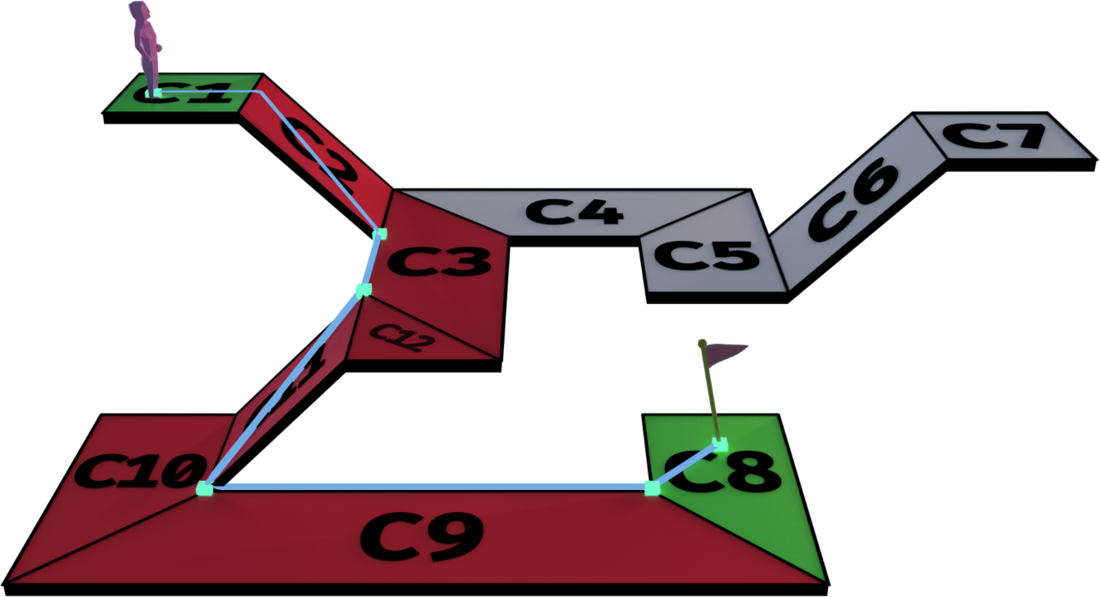
\includegraphics[width=0.9\textwidth]{images/mesh_with_path.png}
	\caption{Von \cite{Mesh:18}: Navigation Mesh mit einem Pfad von Startpunkt C1 bis Endpunkt C8.}
	\label{sec1b}
\end{figure}


\section{Rastergraph (\textit{eng.} Grid Graph)}
%A Star is good for them
%Grids are composed of tiles which lie adjacent to each other
%A raster is put on top of the environment where it will be used. Then a Graph Search with its Tiles is used to find a path in it. For that each Tile possess a travel cost. A common Pathfinding Algorthim used here is A*.
%A common Tile has 4 adjacent Tiles, however more options for a grid are possible. A hextile has six neighbours and the Octile has eight, 4 adjacent like the regular tile and 4 from diagonal movement.
%(1)
Raster bestehen aus Kacheln, die nebeneinander liegen. Laut \cite{Grid:02} wird ein Raster wird "uber die Umgebung gelegt, in der er genutzt werden soll. Dann wird eine Graphensuche verwendet, um einen Pfad darin zu finden. Daf"ur besitzt jede Kachel seine eigenen Kosten. Die Kacheln sind Knoten und jede hat Kanten zu ihren Nachbarn. Ein "ublicher Pfadfindungsalgorithmus daf"ur ist A*.
\\\\
F"ur den Graph hat eine Kachel typischerweise vier benachbarte Kacheln, es sind jedoch mehr Optionen m"oglich. Eine sechseckige Kachel hat sechs Nachbarn und die normale rechteckige Kachel hat dann acht, wenn die Diagonalen betrachtet werden (siehe Abb. \ref{sec2a}).
\begin{figure} %Gemacht mit Paint
	\centering
	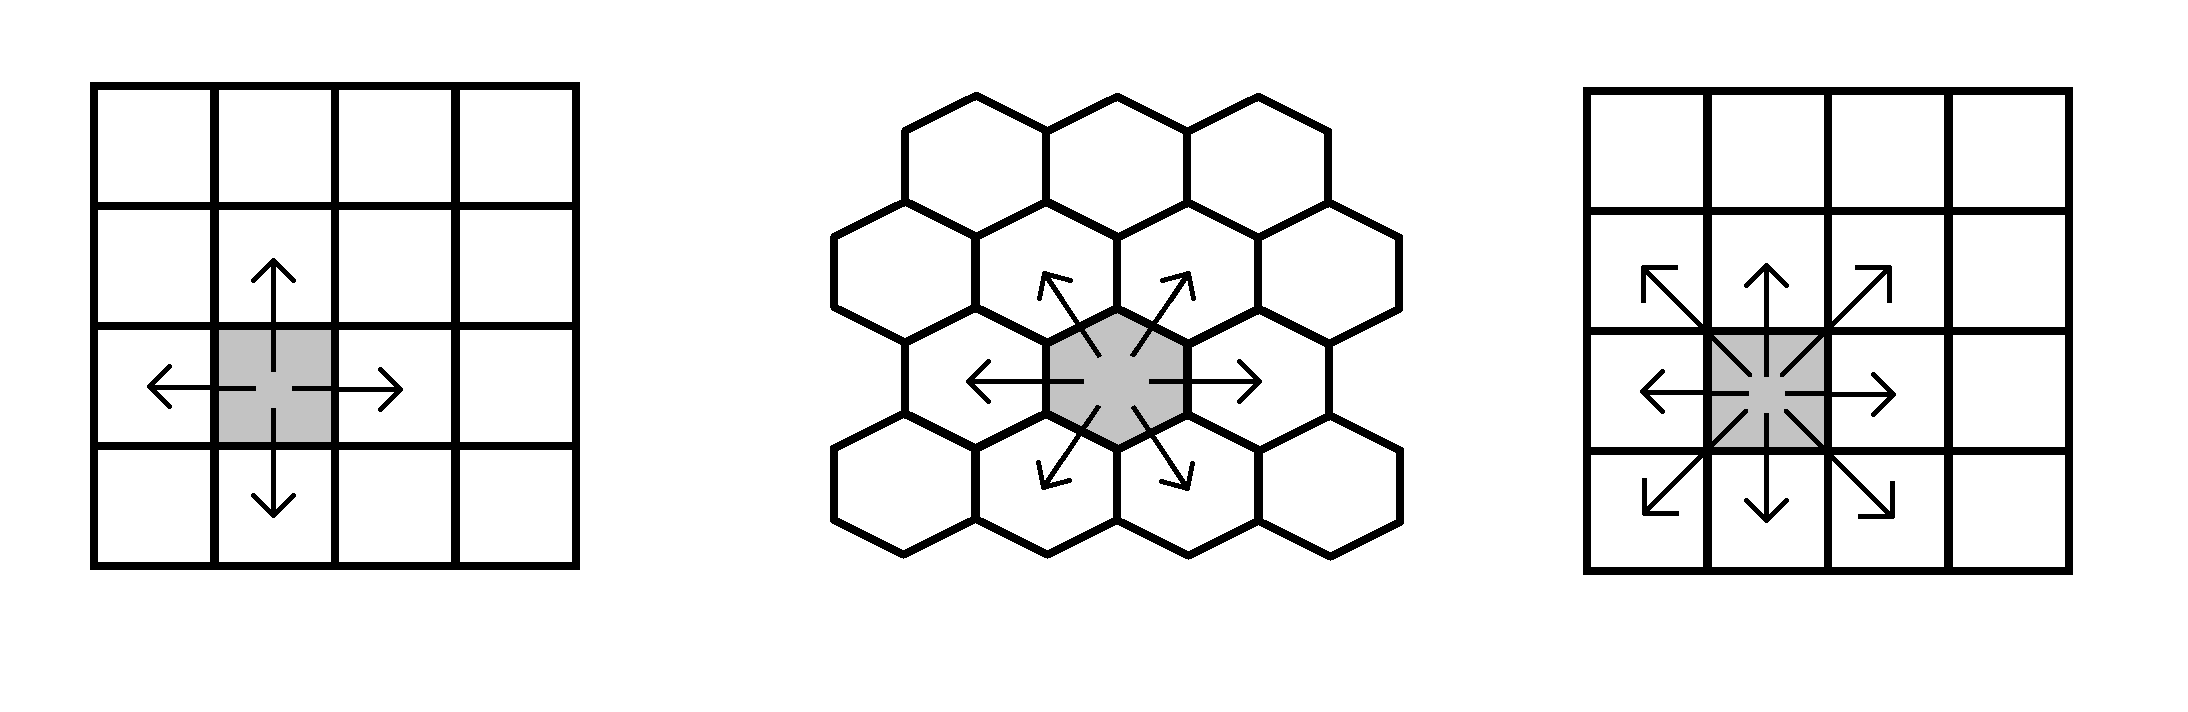
\includegraphics[width=\textwidth]{images/Grid_Tiles.png}
	\caption{Von links nach rechts: Kachel mit 4 Bewegungsoptionen, Hexagon mit 6 Bewegungsoptionen, Kachel mit 8 Bewegungsoptionen.}
	\label{sec2a}
\end{figure}


\section{Sichtbarkeitsgraph (\textit{eng.} Visibility Graph)}
%(110)
%The defining characteristics of a visibility map are that its nodes share an edge if they
%are within line of sight of each other, and that all points in the robot’s free space are
%within line of sight of at least one node on the visibility map.
%
%The standard visibility graph is defined in a two-dimensional polygonal configuration
%space (figure 5.3). The nodes vi of the visibility graph include the start location,
%the goal location, and all the vertices of the configuration space obstacles. The graph
%edges ei j are straight-line segments that connect two line-of-sight nodes vi and vj , i.e.,
%Proper Work
%(110)
%Visibility graphs consist of nodes that share an edge if they are withhin line if sight with each other and no obstacle lies between them. The standard Graph is two dimensional. Possesing the start point, end point and the vertices of the polygons that represent obstacles as nodes.
%
%An example of a visibility graph lies in image ref.
%(110)
In \cite{Principles:05} ist beschrieben, dass Sichtbarkeitsgraphen aus Knoten bestehen, die in Sichtlinie der Roboter stehen. Eine Kante zwischen zwei Punkten gilt nur, wenn keine Hindernisse zwischen ihnen liegt. Der Standardgraph ist zweidimensional. Der Startpunkt und der Endpunkt werden als Knoten dargestellt, sowie die Eckpunkte der Polygone, die Hindernisse darstellen.
\\\\
Ein Beispiel f"ur einen Sichtbarkeitsgraphen findet sich in Bild \ref{sec3a}.
\begin{figure} %Genommen aus Buch
	\centering
	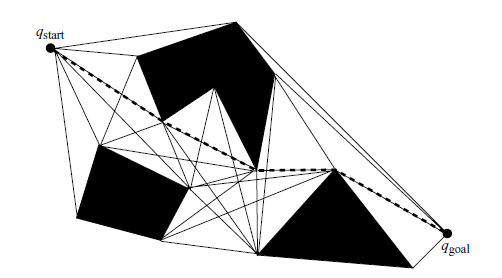
\includegraphics[width=\textwidth]{images/Robot_Motion_Visibility_Graph.png}
	\caption{Von \cite[~S. 111]{Principles:05} \textit{Figur 5.4} Die Linien begrenzen die Kanten des Sichtbarkeitsgraphen f"ur die drei, als gef"ullte Polygone dargestellten Hindernisse. Die gepunktete Linie, stellt den k"urzesten Weg zwischen Start und Ziel dar.}
	\label{sec3a}
\end{figure}


%\section{Adjacency graph}
%%bbbb
%
%\section{Punktgraphen (Point Graphs)}
%
%
%\section{(Automatic Navmesh Calculation)}
%
%
%\subsection{Zerteilung des Navmesh (Navmesh Cutting)} 